\chapter{Design and Analysis} \label{cha:design}
In this chapter the design of SeriChat, which aims to fulfill the requirements defined in \autoref{cha:introduction}, is presented.

\section{System Overview}
The group chat system, SeriChat, consists of two layers. The first layer is the Kademlia infrastructure based on the TomP2P implementation. The second layer implements the extension with group functionality on top of TomP2P. This layer uses the standard Kademlia functionalities, but it also in some cases communicate using extra features outside of Kademlia. 

\section{Group Communication}
Group Communication is created by building a separate tree-structure. The tree-structure is build as a binary-tree where the root is the \emph{GroupOwner}. In some P2P group chat designs like SCRIBE, the root is always the \emph{GroupInfoHolder}. However SeriChat focuses on fairness and thus we have chosen to not put unnecessary load or responsibility on a specific node in the group. The same is valid for the concept of \emph{forwarder} in SCRIBE, were nodes that are not members of the group can act as \emph{forwarder}. It is not fair to load a node which is not a member of a certain group and therefore we have chosen to design this part differently from SCRIBE.

In the following subsections the design of four scenarios in group chatting is presented. These scenarios are: \emph{create}, \emph{join}, \emph{leave} and \emph{communicate}.

\subsection{Create}
When a node choose to create a group it puts an entry in the DHT. The entry has a key consisting of the hashes of the \emph{GroupName} and a value consisting of information about the group, like the ip-address, the node-id, and the public-key of the root. The node which holds this entry is called \emph{GroupInfoHolder} as illustrated in \autoref{fig:createScenario}. The \emph{GroupOwner} lastly generates an \emph{AES} secret-key for the newly created group and store it inside itself.

\begin{figure}[bth]
	\centering
	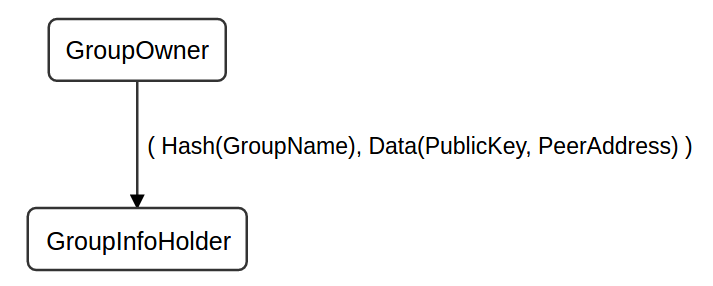
\includegraphics[width=0.7\linewidth]{gfx/createScenario}}
	\caption{Create scenario}
	{\label{fig:createScenario}
\end{figure}


\subsection{Join}
When a node choose to join a group, it looks up the hashes of the \emph{GroupName} to get informations needed for joining the group. It then uses the received value to send a joining event directly to the root containing the password needed to be authorized by the root which is also the \emph{GroupOwner}. Both the \emph{GroupName} and the password has to be obtained from outside the SeriChat. If the authorizing was successful the root replies with the \emph{GroupSecretkey}. \autoref{fig:joinScenario} illustrates the join scenario.

\begin{figure}[bth]
	\myfloatalign
	\subfloat[Get group info]
	{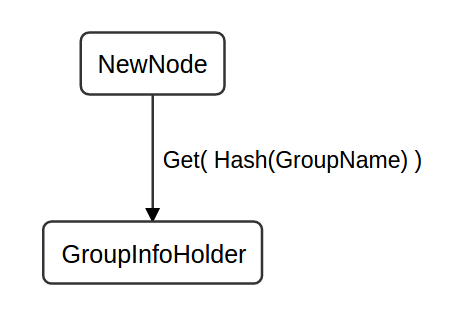
\includegraphics[width=.45\linewidth]{gfx/joinScenario1}} \quad
	\subfloat[Send join event to the GroupOwner]
	{\label{fig:example-b}%
		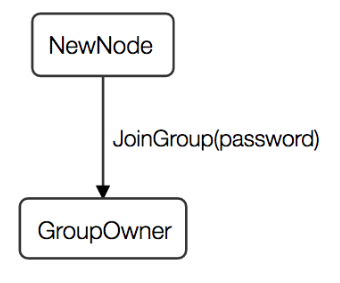
\includegraphics[width=.35\linewidth]{gfx/joinScenario2}} \\
	\caption{Join scenario}\label{fig:joinScenario}
\end{figure}

It is clear that SeriChat uses the top-down approach in the join scenario. The top-down approach gives the opportunity to balance the binary-tree, which is important for the performance. The root and the members, in the top-down approach, have the decision about where new members should be placed. The algorithm used for the placement is fairly simple. Every time a root or a member forwards a new member to the children, the choice is the inverse of the previous choice. This results in a balanced tree because the members are always switching between forwarding to the right-child or forwarding to the left-child. 

\subsection{Leave}
When a peer choose to leave the group it informs its children by sending a \emph{leave event}. The children will then inform the root about their parent's leaving together with a \emph{rejoin event}. The system finds a new place for them by use of the same algorithm described in the join scenario.
%figure ??? 

\subsection{Communicate}
When a node choose to send a message to its group members a \emph{forward-message event}, containing the message itself,  is sent directly to the root. The root reads the message and forwards it to the children by using the same \emph{forward-message event}. The children also reads the message and forwards the event and so on and so forth.

SeriChat also uses the top-down approach in this scenario. The reason for that is that the top-down approach ensures a correct order of receiving the messages for all the members without any extra overhead.

\autoref{fig:forwardMsg} illustrates the communication scenario.
\begin{figure}[bth]
	\myfloatalign
	\subfloat[Forwards to the root]
	{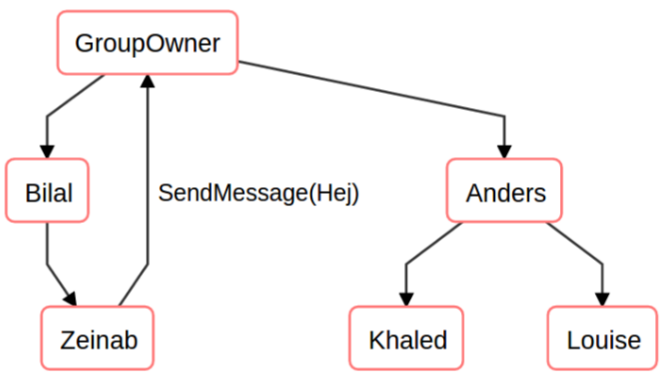
\includegraphics[width=.45\linewidth]{gfx/forwardMsg1}} \quad
	\subfloat[Forwards to the rest of the group]
	{\label{fig:example-b}%
		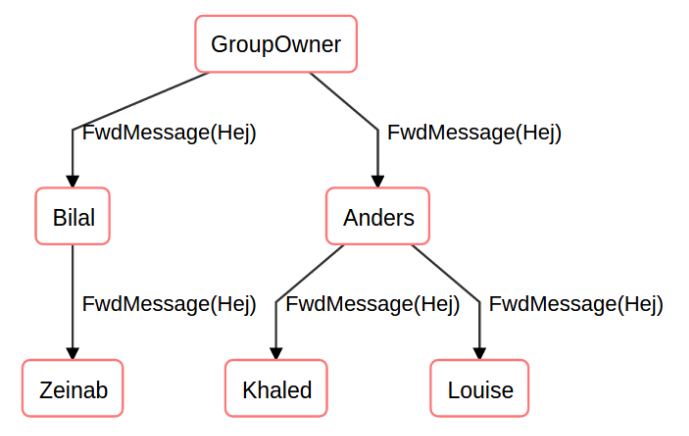
\includegraphics[width=.45\linewidth]{gfx/forwardMsg2}} \\
	\caption{Communicate scenario}\label{fig:forwardMsg}
\end{figure}

\section{Fault-tolerance}
Fault-tolerance in the Kademlia infrastructure is ensured by TomP2P, but the tree-structure for the group communication is not. The tree-structure is vulnerable because the members depends on each other to fulfill the communication and a single failure can have a huge impact especially when it is the root that fails. Fault-tolerance for the tree-structure should therefore be ensured. In the following subsections the design of handling two different failure scenarios, in group chatting, is presented. These scenarios are: \emph{failed root} and \emph{failed member} and are both inspired by \cite{matl2015effective}.

\subsection{Failed Root}
When a root fails one of the group members has to take over as soon as possible.
The \emph{GroupOwner} chooses therefore one or two of the members and makes them the co-owners. The co-owners receives a replication of the \emph{GroupOwner}'s data and are placed at the same level as the root as illustrated in \autoref{fig:failedRoot}. The co-owners have to monitor the \emph{GroupOwner} and take over the job (one of them) when necessary. The monitoring is done by sending \emph{``heartbeat'' events} \cite{aguilera1997heartbeat} periodically from the \emph{GroupOwner} to the co-owners. Thereby the co-owners are able to indicate a failed root as soon as the \emph{heartbeat events} are interrupted.

\begin{figure}[bth]
	\centering
	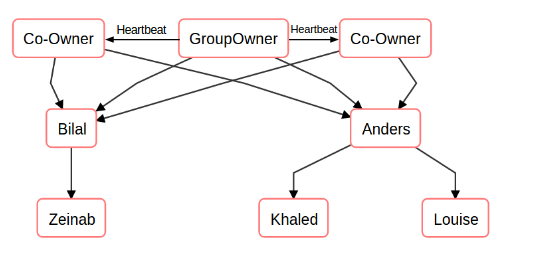
\includegraphics[width=0.7\linewidth]{gfx/failedRoot}}
\caption{Failed Root Scenario}
{\label{fig:failedRoot}
\end{figure}


\subsection{Failed Member}
When a group member fails its children have to rejoin the group as soon as possible. Every parent therefore sends \emph{heartbeat events} periodically to their children. Thereby the children are able to indicate a failed parent as soon as the \emph{heartbeat events} are interrupted. When a failure is indicated the children will act as if they received a \emph{leave event}.

\begin{figure}[bth]
	\centering
	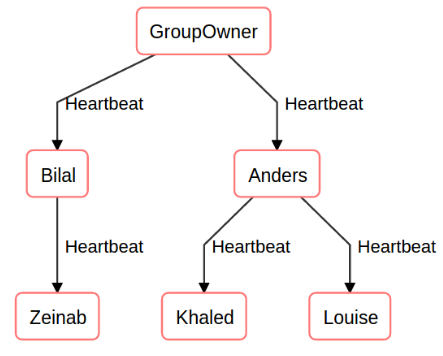
\includegraphics[width=0.6\linewidth]{gfx/failedMember}}
\caption{Failed Member Scenario}
{\label{fig:failedMember}
\end{figure}

\section{Confidentiality}
To ensure confidentiality it is important to treat two cases in the group chat. The first case is when a node joins a group the communication between the joining peer and the root have to be kept secret. As the communication is only between two peers it made most sense to use asymmetric encryption. For this asymmetric encryption the RSA algorithm is used by encrypting the password using the public key for the Group Owner. See the illustration on \autoref{fig:jon-enc}.
\begin{figure}[bth]
	\centering
	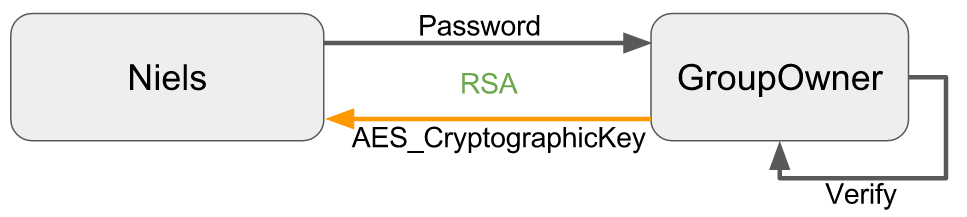
\includegraphics[width=1\linewidth]{gfx/join-enc}}
\caption{RSA encryption in the join-scenario}
{\label{fig:jon-enc}
\end{figure}

The second case is when a message is sent inside the group, where this message should stay private such that only the group members can read the message. In this case the communication is between one to many and thereby its chosen to use symmetric encryption. For symmetric  encryption the AES algorithm is used. An AES cryptographic key is received by each member joining the group. All messages between the groups are encrypted by the known AES cryptographic key. See the illustration on \autoref{fig:comm-enc}.
\begin{figure}[bth]
	\centering
	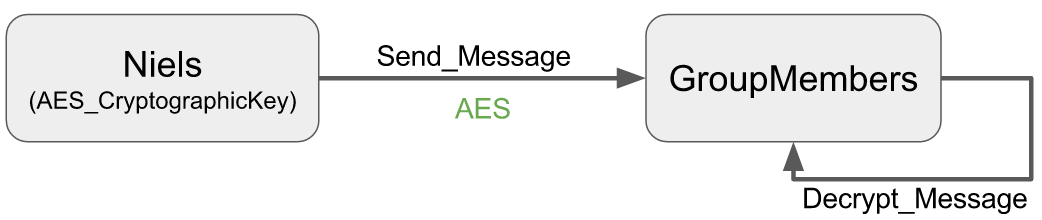
\includegraphics[width=1\linewidth]{gfx/communicate-enc}}
\caption{AES encryption in the communication-scenario}
{\label{fig:comm-enc}
\end{figure}


%TODO: What about deffie-hellman?

%Many of the other natural sciences have labs with equipment that has
%to be configured correctly to experimentally test stated hypotheses.
%Such experiments must be planned and designed in advance to work
%properly and provide valid and trustworthy results.
%
%As computer scientists, we usually do not work in labs, and our
%experiments do not live in petri dishes. Still, we have hypotheses to
%test, and thus, experiments to plan. This planning phase is the
%design, where the authors describe the system intended to test the
%hypotheses posed in the introduction.
%
%A luxury of the design chapter is that the design may well go further
%than solely the confirmation or refutation of the hypotheses.  If you
%are building a system, this is where you show that you know how to
%design one, even if you will actually not be implementing all of it.
%If you had sufficient time and resources, this is how you would make
%your system.
%
%However, before we come to that, it is necessary to investigate
%whether the required hypotheses are valid. If they are not, the design
%must be reconsidered, and there is only one way to test them, namely
%through implementation, and subsequent evaluation.
